\begin{name}
	{\tenchude}{ĐỀ ÔN TẬP SỐ 5}{LỚP TOÁN THẦY PHÁT}{\thoigian}
\end{name}
\setcounter{ex}{0}
\setcounter{bt}{0}
\Opensolutionfile{ans}[ans/ans-Vted-15-2023]
%%==========Câu 1
\begin{ex}%[2D1Y2-2]%Câu 1
	Cho hàm số $y=f(x)$ có bảng xét dấu đạo hàm như sau
	\begin{center}
		
\begin{tikzpicture}
			\tkzTabInit[nocadre=false,lgt=1.2,espcl=1.5,deltacl=0.6]
			{$x$ /0.6,$f'(x)$ /0.6}
			{$-\infty$,$-2$,$-1$,$1$,$4$,$+\infty$}
			\tkzTabLine{,-,$0$,+,$0$,-,$0$,+,$0$,-}
		\end{tikzpicture}
	\end{center}
	Số điểm cực trị của hàm số đã cho là
	\choice
	{$1$}
	{$3$}
	{$2$}
	{\True $4$}
	\loigiai{
		Dựa vào bảng xét dấu, ta thấy hàm số đã cho có $4$ điểm cực trị.
	}
\end{ex}
\begin{ex}%[2D1Y5-4]%Câu 2
	Giao điểm của đồ hàm số $y=x^3-3x^2-1$ với trục tung có tung độ là
	\choice
	{$0$}
	{\True $-1$}
	{$1$}
	{$3$}
	\loigiai{
		Tọa độ giao điểm của đồ hàm số $y=x^3-3x^2-1$ với trục tung là nghiệm của hệ
		\begin{eqnarray*}
			\heva{&y=x^3-3x^2-1\\&x=0}
			\Leftrightarrow &\heva{&x=0\\&y=-1.}
		\end{eqnarray*}
	}
\end{ex}
\begin{ex}%[2D4Y1-1]%Câu 3
	Số phức $z=5\mathrm{i}$ có số phức liên hợp là
	\choice
	{$-5$}
	{\True $-5\mathrm{i}$}
	{$5$}
	{$5\mathrm{i}$}
	\loigiai{
		Số phức $z=5\mathrm{i}$ có số phức liên hợp là $-5\mathrm{i}$.
	}
\end{ex}
\begin{ex}%[2H3Y3-3]%Câu 4
	Trong không gian cho đường thẳng $ d\colon \heva{&x=2+t\\&y=-2+2t\\&z=-3-3t}$ đi qua điểm nào dưới đây?
	\choice
	{Điểm $Q(2;2;3)$}
	{\True Điểm $N(2;-2;-3)$}
	{Điểm $M(1;2;-3)$}
	{Điểm $P(1;2;3)$}
	\loigiai{
		Thay tọa độ điểm $Q$ vào phương trình của đường thẳng $d$ ta được:$\heva{&2=2+t\\&2=-2+2t\\&3=-3-3t}\Leftrightarrow\heva{&t=0\\&t=2\\&t=-2.}$\\
		Thay tọa độ điểm $N$ vào phương trình của đường thẳng $d$ ta được:$\heva{&2=2+t\\&-2=-2+2t\\&-3=-3-3t}\Leftrightarrow\heva{&t=0\\&t=0\\&t=0}\Leftrightarrow t=0.$\\
		Thay tọa độ điểm $M$ vào phương trình của đường thẳng $d$ ta được:$\heva{&1=2+t\\&2=-2+2t\\&-3=-3-3t}\Leftrightarrow\heva{&t=-1\\&t=2\\&t=0.}$\\
		Thay tọa độ điểm $M$ vào phương trình của đường thẳng $d$ ta được:$\heva{&1=2+t\\&2=-2+2t\\&3=-3-3t}\Leftrightarrow\heva{&t=-1\\&t=2\\&t=-2.}$\\
		Vậy đường thẳng $d$ đi qua điểm $N$.
	}
\end{ex}
\begin{ex}%[2H2B1-1]%Câu 5
	Cho khối lăng trụ tứ giác đều có độ dài cạnh đáy bằng $2$ và độ dài cạnh bên bằng $6$. Thể tích của khối lăng trụ đã cho bằng
	\choice
	{ $8$}
	{  $72$}
	{$36$}
	{\True$24$}
	\loigiai{
		Diện tích của đáy của lặng trụ là $S=2^2=4$.\\
		Chiều cao của lặng trụ là $h=6$.\\
		Vậy thể tích của lăng trụ đã cho là $V=S\cdot h=24$.
	}
\end{ex}
\begin{ex}%[2D2Y4-1]%Câu 6
	Tập xác định của hàm số $y=\log_2x$ là
	\choice
	{\True$(0;+\infty)$}
	{$\mathbb{R}\setminus \{0\} $}
	{$\mathbb{R}$}
	{$(1;+\infty)$}
	\loigiai{
		Tập xác định của hàm số $y=\log_2x$ là $(0;+\infty)$.
	}
\end{ex}
\begin{ex}%[2D3B1-1]%Câu 7
	$\displaystyle\int\limits\sqrt[3]{x}\mathrm{\,d}x$ bằng
	\choice
	{$-\dfrac{3}{2\sqrt[3]{x^2}}+C$}
	{$\dfrac{1}{3\sqrt[3]{x^2}}+C$}
	{$\dfrac{4}{3}\sqrt[3]{x^4}+C$}
	{\True $\dfrac{3}{4}\sqrt[3]{x^4}+C$}
	\loigiai{
		Ta có  $\displaystyle\int\limits\sqrt[3]{x}\mathrm{\,d}x=\displaystyle\int\limits x^{\tfrac{1}{3}}\mathrm{\,d}x=\dfrac{3}{4}\sqrt[3]{x^4}+C$.
	}
\end{ex}
\begin{ex}%[1D3B3-3]%Câu 8
	Cho cấp số cộng $(u_n)$ với $u_{2021}=1,u_{2023}=9$ khi đó  $u_{2022}$ bằng
	\choice
	{\True$5$}
	{$3$}
	{$4$}
	{$-3$}
	\loigiai{
		Ta có $\heva{&u_{2021}=u_1+2020d\\&u_{2023}=u_1+2022d}\Leftrightarrow \heva{&u_1+2020d=1\\&u_1+2022d=9}\Leftrightarrow \heva{&u_1=-8079\\&d=4.}$\\
		Vậy $u_{2022}=u_1+2021d=5$.
	}
\end{ex}
\begin{ex}%[2D2Y5-1]%Câu 9
	Nghiệm của phương trình $2^{x-5}=8$ là
	\choice
	{$x=-4$}
	{\True$x=8$}
	{$x=4$}
	{$x=1$}
	\loigiai{
		Ta có $2^{x-5}=8\Leftrightarrow x-5=3\Leftrightarrow x=8$.
	}
\end{ex}
\begin{ex}%[2H3Y1-1]%Câu 10
	Trong không gian $Oxyz$, cho véc-tơ $\overrightarrow{a}=(-2;1;3)$ khi đó $2\overrightarrow{a}$ là
	\choice
	{\True $(-4;2;6)$}
	{$(0;3;5)$}
	{$(-4;-1;-1)$}
	{$(4;-2;-6)$}
	\loigiai{
		Ta có $2\overrightarrow{a}=(-4;2;6)$.
	}
\end{ex}


\begin{ex}%[Câu 11]%[]%[2D4Y1-1]
	Trong mặt phẳng toạ độ, điểm $M(-3 ; 2)$ biểu diễn số phức nào dưới đây?
	\choice 
	{\True $z_1=-3+2i$}
	{$z_2=2-3i$}
	{$z_3=-3-2i$}
	{$z_4=2+3i$}
	\loigiai{Điểm $M(-3,2)$ biểu diễn số phức $z=-3+2i$. }
\end{ex}



\begin{ex}%[Câu 12]%[]%[2H2Y1-2]
	Cho hình nón có bán kính đáy $r$ và độ dài đường sinh $l$. Diện tích toàn phần $S_{\text{tp}}$ của hình nón đã cho được tính theo công thức nào dưới đây?
	\choice 
	{\True $S_{\text{tp}}=\pi r(r+l)$}
	{$S_{\text{tp}}=2 \pi r l$}
	{$S_{\text{tp}}=2 \pi r(r+l)$}
	{$S_{\text{tp}}=\pi rl$}
	\loigiai{Ta có: $$S_{\text{tp}}=S_{\text{xq}}+S_{\text{đáy}}=\pi rl + \pi r^2=\pi r(r+l).$$}
\end{ex}


\begin{ex}%[Câu 13]%[]%[2D2Y3-1]
	Với mọi số thực $a$ dương, $\log _2(2a)$ bằng
	\choice 
	{$\dfrac{1}{2} \log _2 a$}
	{\True $\log _2 a+1$}
	{$\log _2 a-1$}
	{$2 \log _2 a$}
	\loigiai{Ta có: $$\log_2(2a)=1+\log_2 a.$$}
\end{ex}

\begin{ex}%[Câu 14]%[]%[2D1Y1-2]
	Cho hàm số $f(x)$ có bảng biến thiên như sau:
	\begin{center}
		
\begin{tikzpicture}
			\tkzTabInit[nocadre=false,lgt=1.2,espcl=2.5,deltacl=0.6]
			{$x$ /0.6,$f’(x)$ /0.6,$f(x)$ /2}
			{$-\infty$,$-1$,$2$,$+\infty$}
			\tkzTabLine{,+,0,-,0,}
			\tkzTabVar{-/$-\infty$,+/$1$,-/$-5$,+/$+\infty$}
		\end{tikzpicture}
	\end{center}
	Hàm số đã cho nghịch biến trên khoảng nào dưới đây?
	\choice 
	{$(-5 ; 1)$}
	{$(-\infty ; 1)$}
	{$(-5 ;+\infty)$}
	{\True $(-1 ; 2)$}
	\loigiai{Dựa vào bảng biến thiên, ta kết luận hàm số đã cho nghịch biến trên $(-1;2)$.}
\end{ex}
\begin{ex}%[Câu 15]%[]%[2H3Y1-1]
	Trong không gian $Oxyz$, mặt phẳng nào dưới đây nhận véctơ $\overrightarrow{a}=(-2 ; 1 ; 3)$ là một véc-tơ pháp tuyến?
	\choice 
	{\True $-2x+y+3z=0$}
	{$2x+y+3z=0$}
	{$2x-y+3z=0$}
	{$x+3y-2z=0$}
	\loigiai{Mặt phẳng $-2x+y+3z=0$ nhận véc-tơ $\overrightarrow{a}=(-2 ; 1 ; 3)$ là 1 véc-tơ pháp tuyến.}
\end{ex}


%%==========Câu 16
\begin{ex}%[Dự án 12-Vted-2023, Võ Thanh Hiệp]%[2D3Y2-1]
	Nếu $\displaystyle\int\limits_{-1}^{3} f(x) \mathrm{\,d}x=-1$ và $\displaystyle\int\limits_{-1}^{3} g(x) \mathrm{\,d}x=3$
	thì $\displaystyle\int\limits_{-1}^3 \left[ 3f(x)+g(x)\right] \mathrm{\,d}x$ bằng
	\choice
	{$8$}
	{\True $0$}
	{$-6$}
	{$6$}
	\loigiai{
		Ta có $\displaystyle\int\limits_{-1}^3 \left[ 3f(x)+g(x)\right] \mathrm{\,d}x=3\displaystyle\int\limits_{-1}^{3} f(x) \mathrm{\,d}x+\displaystyle\int\limits_{-1}^{3} g(x) \mathrm{\,d}x=3\cdot (-1)+3=0$.
	}
\end{ex}

%%==========Câu 17
\begin{ex}%[Dự án 12-Vted-2023, Võ Thanh Hiệp]%[2D2Y6-1]
	Tập nghiệm của bất phương trình $\log_{2}\left(x-1\right)<3$ là
	\choice
	{$\left(1;7\right)$}
	{$\left(-\infty;9\right)$}
	{\True $\left(1;9\right)$}
	{$\left(9;+\infty\right)$}
	\loigiai{
		Ta có $\log_{2}\left(x-1\right)<3\Leftrightarrow \heva{&x-1>0\\&x-1<8}\Leftrightarrow \heva{&x>1\\&x<9}\Leftrightarrow 1<x<9$. \\
		Suy ra tập nghiệm của 	bất phương trình $\log_{2}\left(x-1\right)<3$ là $\left(1;9\right)$.
	}
\end{ex}

%%==========Câu 18
\begin{ex}%[Dự án 12-Vted-2023, Võ Thanh Hiệp]%[2D4Y1-1]
	Môđun của số phức $z=4-2i$	bằng
	\choice
	{$12$}
	{\True $2\sqrt{5}$}
	{$20$}
	{$2\sqrt{3}$}
	\loigiai{
		Ta có $z=4-2i\Rightarrow \left| z\right|=\left| 4-2i\right|=\sqrt{16+4}=2\sqrt{5}$.
	}
\end{ex}

%%==========Câu 19
\begin{ex}%[Dự án 12-Vted-2023, Võ Thanh Hiệp]%[2D3Y1-1]
	Cho hàm số $f(x)=\mathrm{e}^{-2x}+\sin x$. Khẳng định nào dưới đây đúng?
	\choice
	{$\displaystyle\int f(x) \mathrm{\,d}x=-2\mathrm{e}^{-2x}+\cos x+C$}
	{$\displaystyle\int f(x) \mathrm{\,d}x=-\dfrac{1}{2}\mathrm{e}^{-2x}+\cos x+C$}
	{$\displaystyle\int f(x) \mathrm{\,d}x=-2\mathrm{e}^{-2x}-\cos x+C$}
	{\True $\displaystyle\int f(x) \mathrm{\,d}x=-\dfrac{1}{2}\mathrm{e}^{-2x}-\cos x+C$}
	\loigiai{
		Ta có $ \displaystyle\int \left(\mathrm{e}^{-2x}+\sin x \right) \mathrm{\,d}x=
		\displaystyle\int \mathrm{e}^{-2x} \mathrm{\,d}x+
		\displaystyle\int \sin x \mathrm{\,d}x=
		-\dfrac{1}{2}\mathrm{e}^{-2x}-\cos x+C$.
	}
\end{ex}

%%==========Câu 20
\begin{ex}%[Dự án 12-Vted-2023, Võ Thanh Hiệp]%[2D1Y5-1]
	\immini[thm]{
		Cho hàm số $y=ax^4+bx^2+c$ $(a, b, c\in \mathbb{R})$ có đồ thị là đường cong trong hình bên. Giá trị cực tiểu của hàm số đã cho bằng\\
		\choice[2]
		{$-2$}
		{$-1$}
		{\True $-3$}
		{$2$}
	}{
		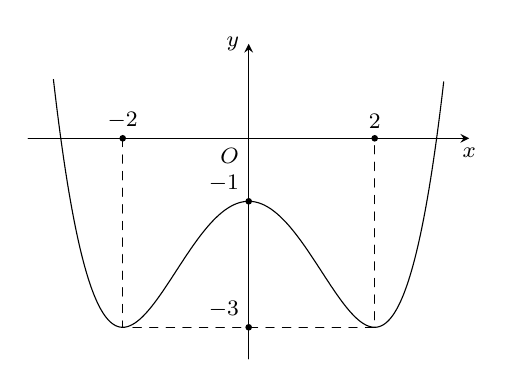
\begin{tikzpicture}[scale=.8,>=stealth, font=\footnotesize, line join=round, line cap=round]
			\def\a{1/8} \def\b{-1} \def\c{-1} % Hệ số
			\draw[->] (-3.5,0)--(3.5,0) node [below]{$x$};
			\draw[->] (0,-3.5)--(0,1.5) node [left]{$y$};
			\node at (0,0) [below left]{$O$};
			\draw[smooth,samples=300,domain=-3.1:3.1] plot(\x,{\a*(\x)^4+\b*(\x)^2+\c});
			\draw[dashed] (-2,0)node [above]{$-2$}|-(0,-3)node [above left]{$-3$}-|(2,0) node [above]{$2$};
			\node at (0,-1) [above left]{$-1$};
			\foreach \i in {(-2,0),(2,0),(0,-1),(0,-3)} \fill \i circle (1.5pt);
		\end{tikzpicture}
	}
	\loigiai{
		Dựa vào đồ thị ta thấy giá trị cực tiểu của hàm số đã cho bằng $-3$.
	}
\end{ex}


\begin{ex}%[Dự án 12-Vted-2023, Võ Thị Thùy Trang]%[1D2Y2-1]%21
	Số hoán vị của tập hợp gồm $10$ phần tử là 
	\choice
	{\True $10!$}
	{$10^2$}
	{$10$}
	{$9!$}
	\loigiai{
		Số hoán vị của tập hợp gồm $10$ phần tử là $10!$.
	}
\end{ex}
\begin{ex}%[Dự án 12-Vted-2023, Võ Thị Thùy Trang]%[2D4B3-2]%22
	Số phức $z$ thỏa mãn $(2-i)\cdot \overline{z}=3-4i$ có phần ảo bằng
	\choice
	{$2$}
	{$-1$}
	{\True $1$}
	{$-2$}
	\loigiai{
		Ta có $(2-i)\cdot \overline{z}=3-4i \Leftrightarrow \overline{z}=\dfrac{3-4i}{2-i}=2-i \Rightarrow z=2+i$.\\
		Suy ra số phức $z$ thỏa mãn $(2-i)\cdot \overline{z}=3-4i$ có phần ảo bằng $1$.
	}
\end{ex}
\begin{ex}%[Dự án 12-Vted-2023, Võ Thị Thùy Trang]%[2D3Y2-1]%23
	Nếu $\displaystyle\int\limits_0^{\frac{\pi}{2}} f(x) \mathrm{\,d}x=-1$ thì $\displaystyle\int\limits_0^{\frac{\pi}{2}} \left[f(x)+\sin x\right] \mathrm{\,d}x$ bằng
	\choice
	{\True $0$}
	{$-\dfrac{\pi}{2}-1$}
	{$-2$}
	{$2$}
	\loigiai{
		Ta có $\displaystyle\int\limits_0^{\frac{\pi}{2}} \left[f(x)+\sin x\right] \mathrm{\,d}x=\displaystyle\int\limits_0^{\frac{\pi}{2}} f(x) \mathrm{\,d}x+\displaystyle\int\limits_0^{\frac{\pi}{2}} \sin x \mathrm{\,d}x=-1-\cos x\bigg|_0^{\frac{\pi}{2}}=-1-(0-1)=0$.
	}
\end{ex}
\begin{ex}%[Dự án 12-Vted-2023, Võ Thị Thùy Trang]%[2D1Y4-1]%24
	Đồ thị hàm số $y=\dfrac{2x-1}{x+1}$ có tiệm cận ngang $y=a$ và tiệm cận đứng $x=b$. Tính tổng $a+b$.
	\choice
	{\True $a+b=1$}
	{$a+b=0$}
	{$a+b2$}
	{$a+b=3$}
	\loigiai{
		Đồ thị hàm số $y=\dfrac{2x-1}{x+1}$ có tiệm cận ngang $y=a$ và tiệm cận đứng $x=b$ nên $a=2$, $b=-1$.\\
		Do đó $a+b=2-1=1$.
	}
\end{ex}
\begin{ex}%[Dự án 12-Vted-2023, Võ Thị Thùy Trang]%[2H3B1-3]%25
	Trong không gian $Oxyz$, cho hai điểm $A(-1;1;-2)$ và $B(3;1;6)$. Phương trình mặt cầu đường kính $AB$ là 
	\choice
	{$(x-1)^2+(y-1)^2+(z-2)^2=80$}
	{$(x+1)^2+(y+1)^2+(z+2)^2=20$}
	{$(x+1)^2+(y+1)^2+(z+2)^2=80$}
	{\True $(x-1)^2+(y-1)^2+(z-2)^2=20$}
	\loigiai{Mặt cầu đường kính $AB$ có tâm $I(1;1;2)$, bán kính $R=\dfrac{1}{2}AB=\dfrac{\sqrt{16+0+64}}{2}=\sqrt{20}$.\\
		Phương trình mặt cầu là $(x-1)^2+(y-1)^2+(z-2)^2=20$.
	}
\end{ex}


%%==========Câu 26
\begin{ex}%[1H3B2-3]
	Cho hình lăng trụ $ABC.A'B'C'$ có tất cả các cạnh bằng nhau. Góc giữa hai đường thẳng $A'C'$ và $BC$ bằng
	\choice
	{$90^\circ$}
	{$30^\circ$}
	{$45^\circ$}
	{\True $60^\circ$}
	\loigiai{
		\immini{
			Ta có $AC\parallel A'C'$ nên góc giữa  $A'C'$ và $BC$ bằng góc giữa  $AC$ và $BC$.\\
			Mà $\triangle ABC$ là tam giác đều nên góc cần tìm là $60^\circ$.
		}
		{
			\begin{tikzpicture}[scale=0.8]
				\def\a{4}
				\def\h{4.5}
				\path 	(0:0) coordinate (A)
				++(0:\a) coordinate (C)
				++(-135:\a/2) coordinate (B)
				($(B)!0.5!(C)$) coordinate (M)
				($(A)!2/3!(M)$) coordinate (G)			
				($(G)+(90:\h)$) coordinate (A')
				($(A')+(C)-(A)$) coordinate (C')
				($(C')+(B)-(C)$) coordinate (B'); 
				\draw[dashed,thick] (A)--(C);
				\draw[thick] (C)--(C') 	(B)--(B') 	(A)--(A') 
				(A)--(B)--(C) (A')--(B')--(C')--cycle;
				\foreach \x/\g in {A/180,B/-135,C/0,A'/180,B'/-160,C'/0}
				\fill[black] 	(\x) circle (1pt)
				($(\g:4mm)+(\x)$) node {$\x$};	
			\end{tikzpicture}
		}
	}
\end{ex}
%%==========Câu 27
\begin{ex}%[2D2Y5-1]
	Với mọi số thực $a,b$ thỏa mãn $2^a\cdot 8^b=16$, khẳng định nào dưới đây đúng?
	\choice
	{$3ab=4$}
	{\True $a+3b=4$}
	{$a^{3b}$=4}
	{$a-3b=4$}
	\loigiai{
		Ta có $2^a\cdot 8^b=16\Leftrightarrow 2^a\cdot 2^{3b} = 2^4\Leftrightarrow 2^{a+3b}=2^4\Leftrightarrow a+3b=4$.	
	}
\end{ex}
%%==========Câu 28
\begin{ex}%[2D1Y3-1]
	\immini{Cho hàm số $f(x) = ax^3+bx^2+cx+d$ có đồ thị như hình vẽ bên. Giá trị nhỏ nhất của hàm số đã cho trên đoạn $[-3;3]$ bằng
		\choice
		{$f(2)$}
		{\True $f(-1)$}
		{$f(-3)$}
		{$f(3)$}
	}
	{
		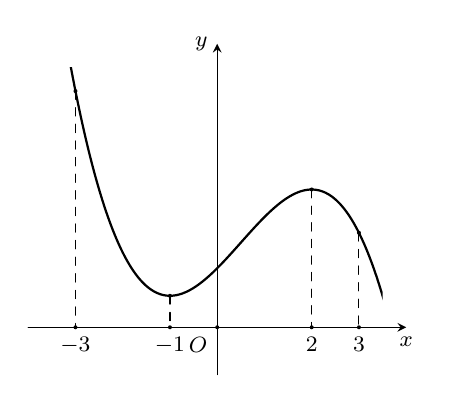
\begin{tikzpicture}[scale=0.6, font=\footnotesize, line join=round, line cap=round, >=stealth]
			\def \xmin{-4};\def \xmax{4};
			\def \ymin{-1};\def \ymax{6};
			\draw[->] (\xmin,0)--(\xmax,0) node[below]{$x$};
			\draw[->] (0,\ymin)--(0,\ymax) node[left]{$y$};
			\fill (0,0) node[below left]{$O$} circle (1.2pt);
			\foreach \x in {-3,-1,2,3} \fill (\x,0) node[below]{$ \x $} circle (1.2pt);
			\clip (\xmin+0.5,\ymin+0.5) rectangle (\xmax-0.5,\ymax-0.5);
			\draw[smooth,thick,samples=100] plot[domain=-3.2:3.6] ({\x},{-(2*(\x)^3-3*(\x)^2-12*\x)/12+1.25});
			\draw[dashed] (-3,5) -- (-3,0) (-1,2/3) -- (-1,0) (2,35/12) -- (2,0) (3,2) -- (3,0);
			\fill (-3,5) circle (1.2pt) (-1,2/3) circle (1.2pt) (2,35/12) circle (1.2pt) (3,2) circle (1.2pt);
		\end{tikzpicture}
	}
	\loigiai{
		Quan sát đồ thị hàm số trên đoạn $[-3;3]$ ta thấy $f(-1)$ là giá trị nhỏ nhất của hàm số.		
	}
\end{ex}
%%==========Câu 29
\begin{ex}%[2H3B2-3]
	Trong không gian $Oxyz$, mặt phẳng qua điểm $M(2;-1;3)$ và vuông góc với trục $Ox$ có phương trình là
	\choice
	{$x+2=0$}
	{$-y+3z=0$}
	{\True $x-2=0$}
	{$z-3=0$}
	\loigiai{
		Mặt phẳng cần tìm đi qua điểm $M(2;-1;3)$ và nhận véc-tơ $\vec{i} = (1;0;0)$ là véc-tơ pháp tuyến nên có phương trình là
		\[ 1(x-2) + 0(y+1) + 0(z-3) = 0\Leftrightarrow x-2=0. \]
	}
\end{ex}
%%==========Câu 30
\begin{ex}%[2D2Y4-2]
	Trên khoảng $(0;+\infty)$, đạo hàm của hàm số $y=x^{\frac{5}{2}}$ là
	\choice
	{$y'=\dfrac{2}{7}x^{\frac{7}{2}}$}
	{$y'=\dfrac{2}{5}x^{\frac{3}{2}}$}
	{\True $y'=\dfrac{5}{2}x^{\frac{3}{2}}$}
	{$y'=\dfrac{5}{2}x^{-\frac{3}{2}}$}
	\loigiai{
		Áp dụng công thức đạo hàm ta có $y'=\dfrac{5}{2}x^{\frac{5}{2}-1} = \dfrac{5}{2}x^{\frac{3}{2}}$.
	}
\end{ex}



\begin{ex}%[2D1Y5-1]
\immini[thm]{Hàm số nào dưới đây có đồ thị như đường cong trong hình bên?\\
	\choice
	{$y=\dfrac{3x+1}{x+2}$}
	{$y=x^2+2x$}
	{$y=2x^3-x^2$}
	{\True $y=x^4-2x^2$}}{
		\begin{tikzpicture}[scale=0.7,>=stealth, font=\footnotesize, line join=round, line cap=round]
			\draw[->] (-2.5,0)--(2.5,0) node[below]{$x$};
			\draw[->] (0,-1.5)--(0,2.5) node[right]{$y$};
			\foreach \u/\v/\z/\t in {0/0/O/45} \fill[black](\u,\v)circle(1pt) ($(\u,\v)+(\t:4mm)$)node{$\z$};
			\clip (-2,-1.5) rectangle (2,2);
			\draw[blue, thick, samples=100] plot(\x,{(\x)^4-2*(\x)^2});
		\end{tikzpicture}}
	\loigiai{
		Từ đồ thị ta có đây là đồ thị của hàm trùng phương, nên đó là đồ thị của hàm số $y=x^4-2x^2$.
	}
\end{ex}
%Câu 32
\begin{ex}%[2D1B1-1]
	Hàm số nào dưới đây đồng biến trên $\mathbb{R}$?
	\choice
	{$y=\dfrac{3x-1}{x+1}$}
	{$y=x^3-x$}
	{$y=x^4-2x^2$}
	{\True $y=x^3+x$}
	\loigiai{
		Xét hàm số $y=x^3+x$ ta có tập xác định $\mathscr{D}=\mathbb{R}$ và $y'=3x^2+1>0,~ \forall x\in\mathbb{R}$.\\
		Vậy hàm số $y=x^3+x$ đồng biến trên $\mathbb{R}$.
	}
\end{ex}
%Câu 33
\begin{ex}%[1H3B5-3]
	\immini{Cho hình hộp $ABCD.A'B'C'D'$ có tất cả các cạnh bằng $6$ và các góc tại đỉnh $A$ đều bằng $60^\circ$ (tham khảo hình bên). Khoảng cách từ $C$ đến mặt phẳng $(A'B'C'D')$ bằng
		\choice
		{$3$}
		{\True $2\sqrt{6}$}
		{$3\sqrt{3}$}
		{$2$}}{\begin{tikzpicture}[scale=0.7, font=\footnotesize, line join=round, line cap=round, >=stealth]
			\path
			(0,0) coordinate (C')
			(5,0) coordinate (A')
			(3,1) coordinate (B')
			($(C')+(A')-(B')$) coordinate (D')
			(2,2) coordinate (C)
			($(C)+(B')-(C')$) coordinate (B)
			($(D')+(C)-(C')$) coordinate (D)
			($(B)+(D)-(C)$) coordinate (A)
			;
			\draw 
			(A)--(B)--(C)--(D)--cycle 
			(C)--(C')--(D')--(A')--(A)
			(D')--(D)
			;
			\draw[dashed] 
			(A')--(B')--(C') (B)--(B')
			;
			\foreach \p/\g in {A/30, B/120, C/170, D/-20, A'/-10, B'/135, C'/180, D'/-30}
			\draw[fill=black] (\p) circle (1pt) node[shift=(\g:3mm)] {$\p$};
	\end{tikzpicture}}
	\loigiai{
		\immini{
			Ta có các góc tại đỉnh $A$ đều bằng $60^\circ$ nên $\widehat{B'C'C}=\widehat{B'C'D'}=\widehat{D'C'C}=60^\circ$.\\
			Mặt khác tất cả các cạnh của hình hộp đều bằng $6$ nên $ \triangle CC'B'$, $\triangle CC'D'$, $\triangle B'C'D'$ là các tam giác đều cạnh bằng $6$.\\
			Khi đó tứ diện $CB'C'D'$ là tứ diện đều, nên gọi $H$ là hình chiếu vuông góc của $C$ lên $(A'B'C'D')$ thì $H$ là trọng tâm $\triangle B'C'D'$.\\
			Ta được $\mathrm{d}\left(C',(A'B'C'D')\right)=CH$.\\
			Tam giác $CHC'$ vuông tại $H$ nên $$CH=\sqrt{C'C^2-C'H^2}=\sqrt{6^2-\left(\dfrac{2}{3}\cdot3\sqrt{3}\right)^2}=2\sqrt{6}.$$}{\begin{tikzpicture}[scale=0.7, font=\footnotesize, line join=round, line cap=round, >=stealth]
				\path
				(0,0) coordinate (C')
				(5,0) coordinate (A')
				(2.5,1) coordinate (B')
				($(C')+(A')-(B')$) coordinate (D')
				(2,3) coordinate (C)
				($(C)+(B')-(C')$) coordinate (B)
				($(D')+(C)-(C')$) coordinate (D)
				($(B)+(D)-(C)$) coordinate (A)
				($(A')!0.5!(C')$) coordinate (O)
				($(C')!2/3!(O)$) coordinate (H)
				;
				\draw 
				(A)--(B)--(C)--(D)--cycle 
				(C)--(C')--(D')--(A')--(A)
				(C)--(D')--(D)
				;
				\draw[dashed] 
				(A')--(B')--(C')--(A') (B)--(B') (C)--(H)
				(C)--(B')--(D')
				;
				\foreach \p/\g in {A/30, B/120, C/170, D/-20, A'/-10, B'/20, C'/180, D'/-30, H/-120}
				\draw[fill=black] (\p) circle (1pt) node[shift=(\g:3mm)] {$\p$};
				\pic[draw,angle radius=6pt]{right angle=C--H--C'};
		\end{tikzpicture}}
	}
\end{ex}
%Câu 34
\begin{ex}%[2H1B3-2]
	Cho khối chóp đều $S.ABCD$ có $AC=4a$ và $SB=\sqrt{6}a$. Thể tích của khối chóp đã cho bằng
	\choice
	{$\dfrac{16\sqrt{2}}{3}a^3$}
	{\True $\dfrac{8\sqrt{2}}{3}a^3$}
	{$16a^3$}
	{$\dfrac{16}{3}a^3$}
	\loigiai{
		\immini{
			$S.ABCD$ là hình chóp đều nên chiều cao hình chóp là $h=SO$.\\
			Tam giác $SBO$ vuông tại $O$ nên $SO=\sqrt{SB^2-BO^2}=\sqrt{\left(\sqrt{6}a\right)^2-(2a)^2}=a\sqrt{2}$.\\
			$AC=4a\Rightarrow AB=\dfrac{AC}{\sqrt{2}}=\dfrac{4a}{\sqrt{2}}=2\sqrt{2}a$.\\
			Diện tích mặt đáy $ABCD$ là $B=\left(2\sqrt{2}a\right)^2=8a^2$.\\
			Thể tích khối chóp $S.ABCD$ là $V=\dfrac{1}{3}Bh=\dfrac{1}{3}\cdot 8a^2\cdot a\sqrt{2}=\dfrac{8\sqrt{2}}{3}a^3$.}{\begin{tikzpicture}[scale=0.8, font=\footnotesize, line join=round, line cap=round, >=stealth]
				\path
				(0,0) coordinate (A)
				(-1.5,-1.5) coordinate (B)
				(4,0) coordinate (D)
				($(B)+(D)-(A)$) coordinate (C)
				(1,3) coordinate (S)
				($(A)!0.5!(C)$) coordinate (O)
				;
				\draw 
				(S)--(B)--(C)--(D)--(S)--(C)
				;
				\draw[dashed] 
				(O)--(S)--(A)--(C)
				(B)--(A)--(D)--cycle
				;
				\foreach \p/\g in {A/170, B/-90, C/-90, D/0, S/90, O/-90}
				\draw[fill=black] (\p) circle (1pt) node[shift=(\g:3mm)] {$\p$};
				\pic[draw,angle radius=9pt]{right angle=S--O--C};
		\end{tikzpicture}}
	}
\end{ex}
%Câu 35
\begin{ex}%[1D2K5-2]
	Cho tập $X=\{-5;-4;-3;-2;-1;1;2;3;4;5\}$. Chọn 2 số phân biệt từ tập $X$. Tính xác suất để tổng 2 số được chọn là một số âm.
	\choice
	{\True $\dfrac{4}{9}$}
	{$\dfrac{5}{9}$}
	{$\dfrac{2}{3}$}
	{$\dfrac{2}{9}$}
	\loigiai{
	Chọn 2 số từ tập $X$ nên không gian mẫu có $n(\Omega)=\mathrm{C}_{10}^2=45$ kết quả đồng khả năng xảy ra.\\
		Gọi biến  cố $A:$ \lq\lq Chọn được 2 số có tổng là một số âm\rq\rq.
		\begin{itemize}
			\item Trường hợp 1: Chọn được cả 2 số đều âm, có $\mathrm{C}_5^2$ cách chọn.
			\item Trường hợp 2: Chọn được 1 số âm và 1 số dương. Để tổng 2 số là một số thì ta có 4 trường hợp để chọn số âm là $-5$; $-4$; $-3$; $-2$. Ứng với chọn số âm $-5$, ta có 4 cách chọn 1 số dương thuộc $\{1;2;3;4\}$. Ứng với chọn số âm $-4$ ta có 3 cách chọn 1 số dương thuộc $\{1;2;3\}$. Ứng với chọn số âm $-3$ ta có 2 cách chọn số dương thuộc $\{1;2\}$. Ứng với chọn số âm $-2$ chỉ có 1 cách chọn số dương là số 1.\\
			Vậy trường hợp 2 có $4+3+2+1=10$ cách chọn.
		\end{itemize}
		Suy ra $n(A)=\mathrm{C}_5^2+10=20$.\\
		Xác suất của $A$ là $\mathrm{P}(A)=\dfrac{n(A)}{n(\Omega)}=\dfrac{20}{45}=\dfrac{4}{9}$.
	}
\end{ex}



\begin{ex}%[2D3B1-1]
	Họ các nguyên hàm của hàm số $ f(x)=\dfrac{\sin^3x+1}{\sin^2x}$ trên khoảng $\left(0;\pi\right)$ là
	\choice
	{\True $-\cos x-\cot x+C$}
	{$\cos x-\cot x+C$}
	{$-\cos x+\cot x+C$}
	{$\cos x+\cot x+C$}
	\loigiai{
		Ta có\\	$$\displaystyle\int{f(x)\mathrm{\,d}x}=\displaystyle\int{\dfrac{\sin^3x+1}{\sin^2x}\mathrm{\,d}x}=\displaystyle\int{\left(\sin x+\dfrac{1}{\sin^2x}\right)\mathrm{\,d}x}=-\cos x-\cot x+C.$$}
\end{ex}

\begin{ex}%[2H3B3-1]%Câu 2
	Trong không gian $ Oxyz$, đường thẳng $d$ là giao tuyến của hai mặt phẳng $\left(\alpha\right)\colon x+2y+z-1=0$ và $\left(\beta\right)\colon x-y-z+2=0$ có một véc-tơ chỉ phương là
	\choice
	{$\vec u_1=\left(1;2;-3\right)$}
	{$\vec u_2=\left(0;-1;3\right)$}
	{\True $\vec u_3=\left(1;-2;3\right)$}
	{$\vec u_4=\left(1;2;3\right)$}
	\loigiai{
		Mặt phẳng $\left(\alpha\right)$ có một véc-tơ pháp tuyến là $\vec n_\alpha=\left(1;2;1\right)$.\\
		Mặt phẳng $\left(\beta\right)$ có một véc-tơ pháp tuyến là $\vec n_\beta=\left(1;-1;-1\right)$.\\
		Vì $ d=\left(\alpha\right)\cap\left(\beta\right)$ nên đường thẳng $ d$ có một véc-tơ chỉ phương $\vec u$ thỏa $\left\{\begin{aligned}
			&\vec u\bot{\vec n_\alpha}\\
			&\vec u\bot{\vec n_\beta}.
		\end{aligned}\right.$ \\
		Suy ra $\vec u=\left[\vec n_\alpha,\vec n_\beta\right]=\left(-1;2;-3\right)=-\left(1;-2;3\right)$.}
\end{ex}
%
\begin{ex}%[2H2K1-4]%Câu 3
	Một thùng đựng nước có dạng hình hộp chữ nhật có chiều cao là $90$ cm, đáy thùng là hình chữ nhật có chiều rộng là $50$ cm và chiều dài là $80$ cm. Trong thùng có chứa nước, mực nước so với đáy thùng có chiều cao là $40$ cm. Khi đặt vào thùng một khối trụ bằng thép có chiều cao bằng chiều cao của thùng và bán kính đáy là $20$ cm theo phương thẳng đứng thì chiều cao của mực nước so với đáy thùng là bao nhiêu?
	\choice
	{\True $58{,}32$ cm}
	{$48{,}32$ cm}
	{$78{,}32$ cm}
	{$68{,}32$ cm}
	\loigiai{
		Giả sử chiều cao mực nước so với đáy thùng lúc sau là $ h$ cm.\\
		Từ giả thiết ta có\\
		Thể tích nước ban đầu + thể tích khối trụ (chiều cao $h$) = thể tích hộp chữ nhật (chiều cao $ h$).\\
		Vậy $$ 80\cdot 50\cdot 40+\pi{20^2}\cdot h=80\cdot 50\cdot h\Leftrightarrow h=\dfrac{400}{10-\pi}\approx 58{,}323\,\,\text{cm}.$$}
\end{ex}
%
\begin{ex}%[2H3K3-2]%Câu 4
	Trong không gian $ Oxyz$, cho điểm $ A\left(2;3;-1\right)$ và mặt phẳng $(P)\colon 2x-y+2z-2=0$.
	Đường thẳng $ d$ qua $A$ cắt trục hoành tại điểm $ M$ và cắt mặt phẳng $(P)$ tại điểm $ N$ sao cho $ A$ là trung điểm $ MN$ có phương trình là
	\choice
	{$\dfrac{x-2}{5}=\dfrac{y-3}{6}=\dfrac{z+1}{-2}$}
	{\True $\dfrac{x-2}{4}=\dfrac{y-3}{3}=\dfrac{z+1}{-1}$}
	{$\dfrac{x-2}{1}=\dfrac{y-3}{6}=\dfrac{z+1}{-2}$}
	{$\dfrac{x-2}{-4}=\dfrac{y-3}{3}=\dfrac{z+1}{-1}$}
	\loigiai{
		Gọi $ M\left(m;0;0\right)\in Ox\Rightarrow N\left(4-m;6;-2\right)$.\\
		Vì $N\in(P)\Leftrightarrow 2\left(4-m\right)-6-4-2=0\Leftrightarrow m=-2$.\\
		nên $\overrightarrow{AM}=\left(-4;-3;1\right)=-\left(4;3;-1\right)$.\\
		Vậy $ AM\colon \dfrac{x-2}{4}=\dfrac{y-3}{3}=\dfrac{z+1}{-1}$.}
\end{ex}
%
\begin{ex}%[2D4G4-2]%Câu 5
	Trên tập số phức, xét phương trình $z^2+az+b=0$ (với $ a,b$ là các tham số thực). Có nhiêu cặp số thực $\left(a;b\right)$ sao cho phương trình đó có hai nghiệm $z_1$, $z_2$ thỏa mãn $\left|z_1+1+i\right|=1$ và $\left|z_2+2-i\right|=1$?
	\choice
	{\True $3$}
	{$2$}
	{$5$}
	{$4$}
	\loigiai{
		\begin{itemize}
			\item Trường hợp 1: Nếu $\Delta=a^2-4b\ge 0$ thì các nghiệm $z_1$, $z_2$ của phương trình là các số thực $ x,y$. Khi đó\\
			$\left\{\begin{aligned}
				&\left|z_1+1+i\right|=1\\
				&\left|z_2+2-i\right|=1
			\end{aligned}\right.\Leftrightarrow\left\{\begin{aligned}
				&\left(x+1\right)^2+1=1\\
				&\left(y+2\right)^2+1=1
			\end{aligned}\right.\Leftrightarrow\left\{\begin{aligned}
				&x=-1\\
				&y=-2
			\end{aligned}\right.\Leftrightarrow\left\{\begin{aligned}
				&-a=x+y=-3\\
				&b=xy=2
			\end{aligned}\right.\Leftrightarrow\left\{\begin{aligned}
				&a=3\\
				&b=2.
			\end{aligned}\right.$
			\item Trường hợp 2: Nếu $\Delta=a^2-4b < 0$ thì các nghiệm $z_1$, $z_2$ của phương trình là các số phức $z_1=x+yi\Rightarrow{z_2}=\bar z_1=x-yi$. Khi đó\\
			$\left\{\begin{aligned}
				&\left|z_1+1+i\right|=1\\
				&\left|z_2+2-i\right|=1
			\end{aligned}\right.\Leftrightarrow\left\{\begin{aligned}
				&\left(x+1\right)^2+\left(y+1\right)^2=1\\
				&\left(x+2\right)^2+\left(y+1\right)^2=1
			\end{aligned}\right.\Leftrightarrow\left\{\begin{aligned}
				&x=-\dfrac{3}{2}\\
				&\left(y+1\right)^2=\dfrac{3}{4}
			\end{aligned}\right.\Leftrightarrow x=-\dfrac{3}{2},y=-1\pm\dfrac{\sqrt 3}{2}.$\\
			$\Rightarrow\left\{\begin{aligned}
				&-a=z_1+z_2=2x=-3\\
				&b=z_1z_2=x^2+y^2=4\pm\sqrt 3
			\end{aligned}\right.\Leftrightarrow\left\{\begin{aligned}
				&a=3\\
				&b=4\pm\sqrt 3.
			\end{aligned}\right.$\\
		\end{itemize}
		Vậy có 3 cặp số phức $\left(a;b\right)$ thỏa mãn bài toán.}
\end{ex}




\begin{ex}%[Câu 41]%[]%[2D2K6-5]
	Có bao nhiêu số nguyên dương $y$ sao cho ứng với mỗi $y$ có đúng 4 số nguyên $x$ thoả mãn $\log _2 x \cdot \log _3\left(\dfrac{6 x}{y}\right) \leq 0$ ?
	\choice 
	{7 }
	{13}
	{\True 6}
	{12}
	\loigiai{
		Điều kiện: $x>0 ; y>0$. Biền đồi về cùng một cơ số chẳng hạn cơ số 2
		$$
		\log _2 x \cdot \log _3 2 \log _2\left(\dfrac{6 x}{y}\right) \leq 0 \Leftrightarrow \log _2 x\left(\log _2 x-\log _2\left(\dfrac{y}{6}\right)\right) \leq 0(*)
		$$
		\\ \textbf{Trường hợp 1.}\\ Nếu $\log _2\left(\dfrac{y}{6}\right)=0 \Leftrightarrow y=6 \Rightarrow(*) \Leftrightarrow \log _2 x=0 \Leftrightarrow x=1 \Rightarrow S_x=\{1\}$ (loại).
		\\ \textbf{Trường hợp 2.}\\ Nếu $\log _2\left(\dfrac{y}{6}\right)>0 \Leftrightarrow \dfrac{y}{6}>1 \Rightarrow(*) \Leftrightarrow 0 \leq \log _2 x \leq \log _2\left(\dfrac{y}{6}\right) \Rightarrow S_x=\left[1 ; \dfrac{y}{6}\right]$ chứa đúng 4 số nguyên $x$ là các số $1, \ldots, 4 \Leftrightarrow 4 \leq \dfrac{y}{6}<5 \Rightarrow y \in\{24, \ldots, 29\}$.
		\\ \textbf{Trường hợp 3.}\\ Nếu $\log _2\left(\dfrac{y}{6}\right)<0 \Leftrightarrow 0<\dfrac{y}{6}<1 \Rightarrow(*) \Leftrightarrow \log _2\left(\dfrac{y}{6}\right) \leq \log _2 x \leq 0 \Rightarrow S_x=\left[\dfrac{y}{6} ; 1\right] \subset[0 ; 1]$ (loại).
		\\Vậy $y \in\{24, \ldots, 29\}$.}
\end{ex}
\begin{ex}%[Câu 42]%[]%[2D4G5-1]
	Xét hai số phức $z_1, z_2$ thoả mãn $\left|z_1-1-i\right|=1 ;\left|z_2-2+i\right|=2$ và số phức $z$ sao cho $\left(z-z_1\right)\left(\overline{z-z_2}\right)$ là số thực; $\left(\overline{z-z_1}\right)\left(1+i-z_1\right)$ và $\left(\overline{z-z_2}\right)\left(2-i-z_2\right)$ là các số thuần ảo. Giá trị nhỏ nhất của $P=|z-3-2 i|$ bằng
	\choice 
	{3}
	{2}
	{0}
	{\True 1}
	\loigiai{
		\\Ta có $\left|z_1-1-i\right|=1 \Rightarrow A\left(z_1\right) \in\left(\mathrm{C}_1\right)$ có tâm $I_1(1 ; 1), R_1=1$ và $\left|z_2-2+i\right|=2 \Rightarrow B\left(z_2\right) \in\left(\mathrm{C}_2\right)$ có tâm $I_2(2 ;-1), R_2=2$. \\Gọi $M(z)$ khi đó $\left(z-z_1\right)\left(\overline{z-z_2}\right)$ là số thực nên $M \in A B$.
		\\Và $\left(\overline{z-z_1}\right)\left(1+i-z_1\right)=\left(\overline{z_1-z}\right)\left(z_1-(1+i)\right)$ là số thuần ảo nên $A M \perp A I_1$
		\\Và $\left(\overline{z-z_2}\right)\left(2-i-z_2\right)=\left(\overline{z_2-z}\right)\left(z_2-(2-i)\right)$ là số thuần ảo nên $B M \perp B I_2$.
		\\Kết hợp ba điều trên suy ra $M$ nằm trên đường thẳng $d$ là tiếp tuyến chung của hai đường tròn $\left(\mathrm{C}_1\right)$ và $\left(\mathrm{C}_2\right)$.
		
		\begin{center}
			\begin{tikzpicture}[scale=1,>=stealth, font=\footnotesize, line join=round, line cap=round]
				\path
				(1,1) coordinate (I1)
				(2,-1) coordinate (I2)
				(0,3) coordinate (S)
				(3,2) coordinate (C)
				(0,2) coordinate (K)
				($(I1)+(180:1)$) coordinate (M)
				($(I2)+(180:2)$) coordinate (N)
				($(I2)!(M)!(S)$) coordinate (P)
				($(I2)!(N)!(S)$) coordinate (Q)
				($(M)!2!(P)$) coordinate (M')
				($(N)!2!(Q)$) coordinate (N')
				($(N')!(C)!(S)$) coordinate (H)
				;
				\draw (I1) circle (1) (I2) circle (2);
				\draw (I2) node[left]{$I_2$}--(I1) node[left]{$I_1$}--(S) node[left]{$S$} (N')--(S) (I2)--node[right]{$2$}(N') (I1)--node[right]{$1$}(M') (K)node[left]{$K$}--(C)node[above]{$C$}--(H) node[right]{$H$};
				\draw[->] (-1,0)--(5,0) node [below]{$x$};
				\draw[->] (0,-4)--(0,4) node [left]{$y$};
				\node at (0,0) [below left]{$O$};
				\pic[draw, angle radius=2mm]{right angle=C--H--S};
				\pic[draw, angle radius=2mm]{right angle=C--K--S};
				\foreach \i/\j in{I1,I2,M,M',N,N',K,H,C,S}{\fill [black](\i) circle (1 pt);}
			\end{tikzpicture}
		\end{center}
		Vì $1=R_2-R_1<I_1 I_2=\sqrt{5}<R_1+R_2=3 \Rightarrow\left(\mathrm{C}_1\right),\left(\mathrm{C}_2\right)$ cắt nhau nên tiếp tuyến chung $d$ cắt $I_1 I_2$ tại điểm $S$ thỏa mãn $\overrightarrow{S I_1}=\dfrac{R_1}{R_2} \overrightarrow{S I_2}=\dfrac{1}{2} \overrightarrow{S I_2} \Rightarrow S(0 ; 3) \Rightarrow d: a x+b(y-3)=0$.
		\\Vì $\mathrm{d}\left(I_1, d\right)=R_1 \Leftrightarrow \dfrac{|a-2 b|}{\sqrt{a^2+b^2}}=1 \Leftrightarrow(a-2b)^2=a^2+b^2 \Leftrightarrow 3 b^2-4 a b=0 \Leftrightarrow\hoac{&b=0 \Rightarrow d_1: x=0 \\& 4 a=3 b \Rightarrow d_2: 3 x+4 y-12=0.}$
		\\Gọi $C(3 ; 2)$, khi đó $P=|z-3-2 i|=M C \geq \min \left\{\mathrm{d}\left(C, d_1\right), \mathrm{d}\left(C, d_2\right)\right\}=\min \{3,1\}=1$.}
\end{ex}



%%==========Câu 43
\begin{ex}%[Dự án 12-Vted-2023, Võ Thanh Hiệp]%[2H1K3-4]
	Cho khối lăng trụ $ABC.A'B'C'$ có hình chiếu vuông góc của $A'$ lên mặt phẳng $\left(ABC\right)$ là trung điểm $M$ của cạnh $AC$. Biết tam giác $MBC$ vuông cân tại $B$, khoảng cách từ $A$ đến mặt phẳng $\left(A'BC\right)$ bằng $2a$. Góc giữa mặt phẳng $\left(A'BC\right)$ và đáy bằng $45^{\circ}$. Thể tích khối lăng trụ đã cho bằng
	\choice
	{\True $2\sqrt{2} a^3$}
	{$\sqrt{2} a^3$}
	{$3\sqrt{2} a^3$}
	{$\dfrac{2\sqrt{2} a^3}{3}$}
	\loigiai{
		\begin{center}
			\begin{tikzpicture}[scale=1]%lăng trụ tam giac
				\begin{scope}
					%\draw[color=gray!50,dashed] (-2,-2) grid (6,4);
					\def\x {4.5}  \def\y {3.5}  \def\h {3.5}
					\path
					(0,0) coordinate (A)
					($(A)+(0:\x)$) coordinate (C)
					($(A)+(-20:\y)$) coordinate (B)
					($(A)!.5!(C)$) coordinate (M)
					($(M)+(90:\h)$) coordinate (A')
					($(A')+(0:\x)$) coordinate (C')
					($(A')+(-20:\y)$) coordinate (B')
					($(A')!.5!(B)$) coordinate (H)
					;
					\draw (A)--(B)--(C) (A')--(B')--(C')--cycle (A)--(A') (B)--(B') (C)--(C') (A')--(B);
					\draw[dashed] (A)--(C)--(A')--(M)--(B) (M)--(H);
					\pic [draw,angle radius=2mm] {right angle=C--B--M};
					\pic [draw,angle radius=2mm] {right angle=M--H--B};
					\pic [draw,angle radius=2mm] {right angle=B--M--A'};
					\foreach \i/\j in{A/-150,B/-60,C/-60,A'/150,B'/80,C'/30,M/150,H/60}{\fill [black](\i) circle (1pt) ($(\i)+(\j:3mm)$) node {\i};}
				\end{scope}
			\end{tikzpicture}
		\end{center}
		Ta có 	$M$ là trung điểm của cạnh $AC$, $C\in\left(A'BC\right)$ nên $\mathrm{d}\left(A,(A'BC)\right)=2\mathrm{d}\left(M,(A'BC)\right)=2a\Leftrightarrow \mathrm{d}\left(M,(A'BC)\right)=a$.\\
		Vì $SM\perp(ABC)$, $MB\perp BC$ nên $SB\perp BC\Rightarrow BC\perp (A'MB)$.\\
		Kẻ $MH\perp A'B,  (H\in A'B)\Rightarrow MH\perp (A'BC)\Rightarrow MH=\mathrm{d}\left(M,(A'BC)\right)=a$\\
		$\heva{&(A'BC)\cap (ABC)=BC\\& MB\perp BC, MB\subset (ABC)\\&A'B\perp BC, A'B\subset (A'BC)}\Rightarrow $ góc giữa $(A'BC)$ và $(ABC)$ bằng góc $\widehat{A'BM}=45^{\circ}$.\\
		Do đó $\triangle A'MB$ vuông cân tại $M$ và $\triangle MHB$ vuông cân tại $H$.\\
		Suy ra $A'M=MB=MH\sqrt{2}=a\sqrt{2}$.\\
		Vì vậy $V_{ABC.A'B'C'}=S_{\triangle ABC}\cdot A'M=2S_{\triangle BCM}\cdot A'M=MB\cdot BC\cdot A'M=a\sqrt{2}\cdot a\sqrt{2}\cdot a\sqrt{2}=2\sqrt{2} a^3$.
	}
\end{ex}

%%==========Câu 44
\begin{ex}%[Dự án 12-Vted-2023, Võ Thanh Hiệp]%[2H2K1-3]
	Cho hình nón đỉnh $S$ và có đáy là hình tròn tâm $O$. Biết rằng chiều cao của nón bằng $a$, bán kính đáy của nón bằng $2a$. Mặt phẳng $\left(P\right)$ đi qua đỉnh $S$ và cắt nón theo dây cung $AB=2\sqrt{3}a$. Diện tích mặt cầu ngoại tiếp tứ diện $SOAB$ bằng
	\choice
	{$5\pi a^2$}
	{\True $17\pi a^2$}
	{$7\pi a^2$}
	{$26\pi a^2$}
	\loigiai{
		\begin{center}
			\begin{tikzpicture}[scale=1]
				\def\h{3}
				\def\a{2}
				\def\b{1}
				\begin{scope}
					\path
					(0,0) coordinate (O)
					($(O)+(0,\h)$) coordinate (S)
					($(O)+(10:\a cm and \b cm)$) coordinate (M)
					($(O)+(170:\a cm and \b cm)$) coordinate (N)
					($(O)+(-80:\a cm and \b cm)$) coordinate (A)
					($(O)+(50:\a cm and \b cm)$) coordinate (B)
					;
					
					\draw [dashed] (M) arc (10:170:\a cm and \b cm);
					\draw  (M) arc (10:-190:\a cm and \b cm);
					\draw (N)--(S)--(M) (S)--(A);
					\draw[dashed] (S)--node [left]{$a$}(O) (S)--(B)--(A) (A)--(O)--(B);
					\foreach \x/\y in{O/-150,A/-100,S/90,B/-70}{\fill [black](\x) circle (1pt) ($(\x)+(\y:3mm)$) node {$\x$};}
				\end{scope}
			\end{tikzpicture}
		\end{center}
		\parbox{.6\textwidth}{
			$\triangle AOB$ có $OA=OB=2a$, $AB=2\sqrt{3}a$.\\
			$\Rightarrow \cos\widehat{AOB}=\dfrac{OA^2+OB^2-AB^2}{2OA\cdot OB}=-\dfrac{1}{2}\Rightarrow \widehat{AOB}=120^{\circ}$.\\
			Gọi $r$ là bán kính đường tròn ngoại tiếp $\triangle AOB$\\
			$\Rightarrow r=\dfrac{AB}{2\sin \widehat{AOB}}=\dfrac{2\sqrt{3}}{2\sin 120^{\circ}}=2a$.\\
			Gọi $I$ là tâm mặt cầu ngoại tiếp tứ diện $SOAB$.\\
			Vì $SO\perp (OAB)$ nên $h=\mathrm{d}\left(I,(OAB)\right)=\dfrac{1}{2}SO=\dfrac{a}{2}$.\\
			Gọi $R$ là bán kính mặt cầu, ta có $R^2=r^2+h^2=4a^2+\dfrac{a^2}{4}=\dfrac{17a^2}{4}$.\\
			Vì vậy $S=4\pi R^2=17\pi a^2$.
		}\hfill
		\parbox{.4\textwidth}{
			\begin{tikzpicture}[scale=1.5,>=stealth, font=\footnotesize, line join=round, line cap=round]% Cầu ngoại tiếp lăng trụ tam giác
				%\draw[color=gray!50,dashed] (-8,-5) grid (8,6);
				\def \h{1}
				\def \a{1.6}
				\def \b{.2*\a}
				\pgfmathsetmacro{\R}{sqrt(\h*\h+\a*\a)}
				\path
				(0,0) coordinate (I)
				($(O)+(0,-\h)$)coordinate (H)
				($(O)+(0,\h)$)coordinate (I')
				($(H)+(0:\a cm and \b cm)$) coordinate (M)
				($(I')+(0:\a cm and \b cm)$) coordinate (M')
				($(H)+(-150:\a cm and \b cm)$) coordinate (A)
				($(H)+(60:\a cm and \b cm)$) coordinate (B)
				($(H)+(120:\a cm and \b cm)$) coordinate (O)
				($(O)+(0,2*\h)$)coordinate (S)
				($(S)!.5!(O)$) coordinate (K)
				($(O)+(I)-(K)$) coordinate (H)
				;
				
				\draw [dashed,thick] (O)--(A)--(B)--cycle (A)--(S)--(B) (S)--(O)--(I) (K)--(I)--(H)--(O);
				\draw[ dashed] (M) arc (0:180:\a cm and \b cm);%Vẽ cung elip
				\draw (M) arc (0:-180:\a cm and \b cm);%Vẽ cung elip
				\draw[ dashed] (M') arc (0:180:\a cm and \b cm);%Vẽ cung elip
				\draw (M') arc (0:-180:\a cm and \b cm);%Vẽ cung elip
				\draw  (I) circle (\R);
				\foreach \i/\j in{I/120,O/150,A/110,B/60,S/60,H/-60}{\fill [black](\i) circle (1pt) ($(\i)+(\j:2mm)$) node {$\i$};}
				
			\end{tikzpicture}
		}
	}
\end{ex}



\begin{ex}%[Dự án 12-Vted-2023, Võ Thị Thùy Trang]%[2D3G3-1] %Cau 45%
	Cho hàm số $f(x)$ bậc năm có bốn điểm cực trị là $x_1$, $x_2$, $x_3$, $x_4$ sao cho $x_1+x_2+x_3+x_4=1$. Gọi $g(x)$ là hàm bậc ba có đồ thị qua bốn điểm cực trị của đồ thị hàm số $f(x)$. Diện tích hình phẳng giới hạn bởi đường $y=\dfrac{f'(x)}{f(x)-g(x)}$, trục hoành, hai đường thẳng $x=-1$; $x=0$ bằng
	\choice
	{$5\ln 2$}
	{\True $5\ln 5$}
	{$5\ln 6$}
	{$5\ln 3$}
	\loigiai{
		Xét $f(x)=a_nx^n+a_{n-1}x^{n-1}+\cdots\Rightarrow f'(x)=na_nx^{n-1}+(n-1)a_{n-1}x^{n-2}+\cdots$ có $n-1$ điểm cực trị là $x_1, x_2, x_3,\cdots,x_{n-1}$ và $g(x)$ là đường cong qua $n-1$ điểm cực trị của đồ thị hàm số đa thức $f(x)$.
		\\
		Dùng phép chia đa thức ta có
		\\
		$ f(x)=\dfrac{1}{n}\bigg[x+\dfrac{a_{n-1}}{na_n}\bigg]f'(x)+g(x)=\dfrac{1}{n}\bigg[x-\dfrac{1}{n-1}(x_1+x_2+x_3+\cdots+x_{n-1})\bigg]f'(x)+g(x)$, trong đó $x_1, x_2, x_3,\cdots,x_{n-1}$ là các nghiệm của $f'(x)=0\Rightarrow x_1+x_2+x_3+\cdots+x_{n-1}=-\dfrac{(n-1)a_{n-1}}{na_n}$.
		\\
		Vì vậy $\dfrac{f'(x)}{f(x)-g(x)}=\dfrac{n}{x-\dfrac{1}{n-1}(x_1+x_2+x_3+\cdots+x_{n-1})}$.
		\\
		Áp dụng với $n=5$ và $x_1+x_2+x_3+x_4=1\Rightarrow \dfrac{f'(x)}{f(x)-g(x)}=\dfrac{5}{x-\dfrac{1}{4}}$.
		\\
		$\Rightarrow S=\displaystyle\int\limits_{-1}^0\bigg|\dfrac{5}{x-\frac{1}{4}}\bigg|\mathrm{\,d}x=5\ln 5$.
	}
\end{ex}
\begin{ex}%[Dự án 12-Vted-2023, Võ Thị Thùy Trang]%[2D1G5-3]%Cau46%
	Cho hàm số $f(x)$ là hàm bậc ba có bảng biến thiên như sau
	\begin{center}
		
\begin{tikzpicture}
			\tkzTabInit[nocadre=false,lgt=1.2,espcl=2.5,deltacl=0.6]
			{$x$ /0.6, $f'(x)$ /0.6, $f(x)$ /2.5}
			{$-\infty$,$-1$,$2$,$+\infty$}
			\tkzTabLine{,+,$0$,-,$0$,+,}
			\tkzTabVar{-/$-\infty$,+/$1$,-/$-5$,+/$+\infty$}
		\end{tikzpicture}
	\end{center}
	Xét $g(x)=f(f(x)+m)$. Có bao nhiêu giá trị nguyên của $m\in[-10;10]$ để phương trình $g'(x)=0$ có đúng $4$ nghiệm thực phân biệt?
	\choice
	{$11$}
	{$4$}
	{$6$}
	{\True $13$}
	\loigiai{
		Ta có  $g'(x)=f'(x)\cdot f'(f(x)+m)$.
		\\
		$g'(x)=0\Leftrightarrow\left[
		\begin{aligned}
			&f'(x)=0\\
			&f'(f(x)+m)=0
		\end{aligned}
		\right.$
		$\Leftrightarrow\left[
		\begin{aligned}
			&x=-1\\
			&x=2\\
			&f(x)+m=-1\\
			&f(x)+m=2
		\end{aligned}
		\right.$
		$\Leftrightarrow\left[
		\begin{aligned}
			&x=-1\\
			&x=2\\
			&f(x)+1=-m\\
			&f(x)-2=-m.
		\end{aligned}
		\right.$
		\\
		$g'(x)=0$ có $4$ nghiệm phân biệt khi và chỉ khi 
		$\left[
		\begin{aligned}
			&-m<-7\\
			&-m>2
		\end{aligned}
		\right.$
		$\Leftrightarrow\left[
		\begin{aligned}
			&m>7\\
			&m<-2.
		\end{aligned}
		\right.$
		\\
		Vì $m\in[-10;10]\Rightarrow m\in\{-10; -9;\cdots;-1;8;9;10\}$. Vậy có $13$ giá trị nguyên của $m$.
	}
\end{ex}


%%==========Câu 47
\begin{ex}%[2D2G5-5]
	Có bao nhiêu cặp số nguyên dương $(m ; n)$ với $m+n \leq 16$ sao cho tồn tại 4 số thực $x$ thoả mãn
	$$
	x^4-2 m x^2+1=\ln \left(x+\sqrt{x^2+1}\right)^{4 n} ?
	$$
	\choice
	{$43$}
	{ $57$}
	{\True $54$}
	{$66$}
	\loigiai{
		Đưa về phương trình: $x^4-2 m x^2+1=4 n \ln \left(x+\sqrt{x^2+1}\right)$.\\
		Với $m$, $n$ là các số nguyên dương thì đồ thị của hai hàm số $g(x)=x^4-2 m x^2+1$;  $h(x)=4 n \ln \left(x+\sqrt{x^2+1}\right)$ có dạng như hình vẽ
		\begin{center}
			% Đồ thị hàm y=ax^4+bx^2+c. Nếu hệ số lớn cần điều chỉnh hệ trục, vùng lưới, domain và lệnh \clip
			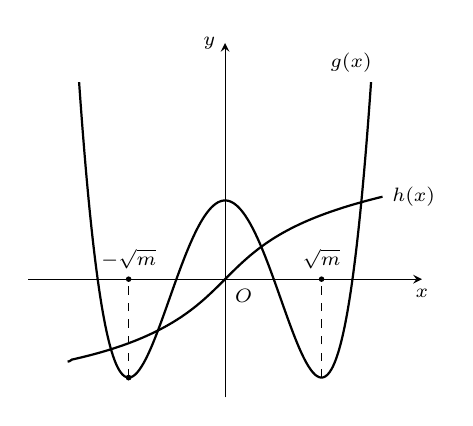
\begin{tikzpicture}[>=stealth,x=1cm,y=1cm,scale=0.5]
				\def\a{1/8} % Hệ số a phải khác 0
				\def\b{-3/2}
				\def\c{2}
				\draw[->] (-5,0) -- (5,0) node[below] {\scriptsize $x$};
				\draw[->] (0,-3) -- (0,6) node[left] {\scriptsize $y$};
				\draw (3.2,5)node[above]{\scriptsize $g(x)$};
				\draw (4,2.094)node[right]{\scriptsize $h(x)$};
				\draw (0,0)node[below right]{\scriptsize $O$};
				\clip (-5,-3)rectangle(5,5);
				\fill[black] (2.45,0)node[above]{\scriptsize $\sqrt{m}$} circle (2pt); 
				\fill[black] (-2.45,0)node[above]{\scriptsize $-\sqrt{m}$} circle (2pt); 
				\fill[black] (-2.45,-2.5) circle (2pt); 
				\fill[black] (-2.45,-2.5) circle (2pt); 
				\draw[thick,samples=150,smooth,domain=-4:4] plot(\x,{\a*(\x)^4+(\b)*(\x)^2+(\c)});
				\draw[thick,samples=150,smooth,domain=-4:4] plot(\x,{ln((\x)+sqrt((\x)^2+1)});
				\draw[dashed] (-2.45,-2.5) -- (-2.45,0) (2.45,-2.5) -- (2.45,0);
			\end{tikzpicture}
			
		\end{center}
		Vậy để phương trình có bốn nghiệm phân biệt $$g(-\sqrt{m})<h(-\sqrt{m}) \Leftrightarrow 1-m^2<4 n \ln (\sqrt{m+1}-\sqrt{m}) \Leftrightarrow n<\dfrac{1}{4 \ln (\sqrt{m+1}-\sqrt{m})}.$$
		Kết hợp với $m+n \leq 16 \Rightarrow 54$ cặp số nguyên dương $(m ; n)$ thoả mãn. \\
		Dò bảng $f(m)=\dfrac{1-m^2}{4 \ln (\sqrt{m+1}-\sqrt{m})}$ trên đoạn $[1 ; 15]$ với Step? bằng 1.\\
		\textbf{TH1:} Nếu $m \in\{1,2\} \Rightarrow f(m)<1 \leq n$ không có cặp số nguyên dương nào thoả mãn.\\
		\textbf{TH2:} Nếu
		\begin{itemize}
			\item $ m=3 \Rightarrow n<1{,}52 \Rightarrow n \in\{1\}$; $m=4 \Rightarrow n<2{,}6 \Rightarrow n \in\{1,2\} $.
			\item $ m=5 \Rightarrow n<3{,}9 \Rightarrow n \in\{1,2,3\} $; $m=6 \Rightarrow n<5{,}4 \Rightarrow n \in\{1, \ldots, 5\} $.
			\item $ m=7 \Rightarrow n<7{,}1 \Rightarrow n \in\{1, \ldots, 7\} $; $m=8 \Rightarrow n<8{,}94 \Rightarrow n \in\{1, \ldots, 8\} $.
			\item $ m=9 \Rightarrow n<10{,}999 \Rightarrow n \in\{1, \ldots, 7\} $; $m=10 \Rightarrow n<13{,}3 \Rightarrow n \in\{1, \ldots, 6\} $.
		\end{itemize}
		\textbf{TH3:} Nếu $ m \in\{11, \ldots, 15\} \Rightarrow f(m)>15 \geq n \Rightarrow n \in\{1, \ldots, 16-m\} \Rightarrow \displaystyle \sum\limits_{m=11}^{15}(16-m)=15$  cặp.\\
		Vậy có tất cả $39+15=54$ cặp số nguyên dương thoả mãn.
	}
\end{ex}

%%==========Câu 48
\begin{ex}%[2D3G2-4]
	Cho hàm số $f(x)$ có đạo hàm liên tục trên $(-\sqrt{2} ; \sqrt{2}) \setminus \{0\}$ thoả mãn $f'(x)+x\left(\mathrm{e}^{f(x)}+2+\mathrm{e}^{-f(x)}\right)=0$. Biết $f(1)=0$, giá trị của $f\left(\dfrac{1}{2}\right)$ bằng
	\choice
	{$\ln 7$}
	{\True $ \ln 5$}
	{$\ln 6$}
	{$\ln 3$}
	\loigiai{
		Biến đổi giả thiết về đúng dạng tích của $f(x)$ và $f'(x)$ :
		$$
		f'(x)+x\left(\mathrm{e}^{f(x)}+2+e^{-f(x)}\right)=0 \Leftrightarrow \dfrac{f'(x)}{\mathrm{e}^{f(x)}+2+\mathrm{e}^{-f(x)}}+x=0 \Leftrightarrow \dfrac{f'(x) \cdot e^{f(x)}}{\left(\mathrm{e}^{f(x)}+1\right)^2}=-x .
		$$
		Cho $f(1)=0$, tính $f\left(\dfrac{1}{2}\right)$ nên ta lấy tích phân hai vế từ $\dfrac{1}{2}$ đến 1 ta được  $\mathrm{V P}=\displaystyle\int\limits_{\frac{1}{2}}^1 -x \mathrm{\,d} x=-\dfrac{3}{8}$.\\
		Tích phân vế trái:
		$$ \mathrm{VT}=\int\limits_{\frac{1}{2}}^1 \dfrac{f'(x) \cdot \mathrm{e}^{f(x)}}{\left(\mathrm{e}^{f(x)}+1\right)^2} \mathrm{\,d} x=\int\limits_{\frac{1}{2}}^1 \dfrac{\mathrm{d}\left(\mathrm{e}^{f(x)}\right)}{\left(\mathrm{e}^{f(x)}+1\right)^2}=-\left.\dfrac{1}{\mathrm{e}^{f(x)}+1}\right|_{\frac{1}{2}} ^1=-\frac{1}{\mathrm{e}^{f(1)}+1}+\frac{1}{\mathrm{e}^{f\left(\frac{1}{2}\right)}+1}=-\frac{1}{2}+\frac{1}{\mathrm{e}^{f\left(\frac{1}{2}\right)}+1} . $$
		Vậy $-\dfrac{1}{2}+\dfrac{1}{\mathrm{e}^{f\left(\frac{1}{2}\right)+1}}=-\dfrac{3}{8} \Leftrightarrow \mathrm{e}^{f\left(\frac{1}{2}\right)}=7 \Leftrightarrow f\left(\dfrac{1}{2}\right)=\ln 7$ .
	}
\end{ex}


%%==========Câu 49
\begin{ex}%[2H3G3-8]
	Trong không gian $Oxyz$, cho hai điểm $A\left(2;\dfrac{9}{2};-2\right)$, $B\left(4;\dfrac{7}{2};0\right)$ và đường thẳng $d\colon \dfrac{x-2}{1}=\dfrac{y-6}{1}=\dfrac{z-1}{4}$. Gọi $(S)$ là mặt cầu có tâm $I$ qua hai điểm $A$, $B$ và tiếp xúc với đường thẳng $d$. Bán kính của $(S)$ có giá trị nhỏ nhất bằng
	\choice
	{\True $\dfrac{6\sqrt{2}-3\sqrt{3}}{2}$}
	{$\dfrac{3\sqrt{2}}{2}$}
	{$\dfrac{4\sqrt{3}-3\sqrt{2}}{2}$}
	{$\dfrac{3\sqrt{3}}{4}$}
	\loigiai{
		Bài toán mặt cầu đi qua hai điểm $A$ và $B$ tiếp xúc với đường thẳng $d$. Về mặt tổng quát hoàn toàn xử lý được thông qua tính toán đại số và giải tích (tham khảo cách 2). Xử lý hình học có thể giải quyết được cho trường hợp $A B$ và $d$ đồng phẳng tức $A B \parallel d$ hoặc $A B \cap d=C$.\\
		Gọi $I$ là tâm và bán kính $R$. Ta có $d \cap A B=C(1 ; 5 ;-3)$.\\
		Vì $I A=I B=R \Rightarrow I \in(P)\colon 2 x-y+2 z=0$ là mặt phẳng trung trực của $A B$ có $E(3 ; 4-1)$ là trung điểm $A B$.\\
		Ta có $I E=\sqrt{R^2-\left(\dfrac{A B}{2}\right)^2}=\sqrt{R^2-\dfrac{9}{4}}$.
		\begin{center}
			\begin{tikzpicture}[scale=0.8, font=\footnotesize, line join=round, line cap=round, >=stealth]
				\path
				(0,0) coordinate (m)
				(1,2) coordinate (n)
				(6,0) coordinate (q)
				($(n)+(q)-(m)$) coordinate (p)
				(5,1) coordinate (E)
				(5,2.5) coordinate (A) 
				($(A)!2!(E)$) coordinate (B)
				(4,0.5) coordinate (I)
				(0.5,-1) coordinate (u) 
				(2,3) coordinate (v)
				(intersection of u--v and m--q) coordinate (x)
				(intersection of A--B and m--q) coordinate (y)
				($(u)!0.5!(v)$) coordinate (M)
				($(u)!(I)!(v)$) coordinate (H)
				;
				\draw 
				(m)--(n)--(p)--(q)--cycle
				(u)--(x) (B)--(y) (M)--(v)node[right]{$d$}
				(E)--(A) (M)--(E)--(I)--(M) (I)--(H)
				;
				\draw[dashed] 
				(x)--(M)
				(y)--(E)
				;
				\foreach \p/\g in {A/90, B/-90, E/0, M/180, H/180, I/-90}
				\draw[fill=black] (\p) circle (1pt) node[shift=(\g:3mm)] {$\p$};
				\pic[draw,angle radius=6pt]{right angle=I--H--v};
				\pic ["$P$",draw,angle radius=6mm]{angle=q--m--n};
			\end{tikzpicture}
		\end{center}
		Ta có $d \cap(P)=M(2 ; 6 ; 1)$ và $ME$ là hình chiếu vuông góc của đường thẳng $d$ lên mặt phẳng $(P)$;\\
		$\overrightarrow{n}_p=(2 ;-1 ; 2)$, $\overrightarrow{u}_d=(1 ; 1 ; 4) \Rightarrow \sin (d,(P))=\dfrac{1}{\sqrt{2}} \Rightarrow(d,(P))=45^\circ$.\\
		Gọi $H$ là hình chiếu vuông góc của điểm $I$ lên đường thẳng $d$.
		\allowdisplaybreaks
		\begin{eqnarray*}
			\Rightarrow R=I H=I M \sin \widehat{H M I} &\geq&(E M-E I) \sin \widehat{H M I}
			=\left(3-\sqrt{R^2-\dfrac{9}{4}}\right) \sin \widehat{H M I}\\ &\geq&\left(3-\sqrt{R^2-\dfrac{9}{4}}\right) \sin 45^0 \\
			\Rightarrow R &\geq& \dfrac{3-\sqrt{R^2-\dfrac{9}{4}}}{\sqrt{2}} \\
			\Rightarrow R &\geq& 3 \sqrt{2}-\dfrac{3 \sqrt{3}}{2}.
		\end{eqnarray*}
		Dấu bằng xảy ra khi $M$, $I$, $E$ thẳng hàng theo thứ tự và $M I=R \sqrt{2}=\left(3 \sqrt{2}-\dfrac{3 \sqrt{3}}{2}\right) \sqrt{2}=6-\dfrac{3 \sqrt{6}}{2}$.\\
		\textbf{Cách 2:} Ta có $I A=I B=R \Rightarrow I \in(P)\colon 2 x-y+2 z=0$ là mặt phẳng trung trực của $A B$ và $(S)$ tiếp xúc với $d$
		$\Rightarrow I \in(Q)\colon x+y+4 z+18 t=0$ (thầy chọn $18 t$ để lát giải hệ tìm giao điểm cho toạ độ gọn hơn chút) là mặt phẳng vuông góc với $d$.\\
		Khi đó $I\left(x ; x-6 t ;-\dfrac{1}{2} x-3 t\right)=(P) \cap(Q)$ và $d \cap(Q)=H\left(-t+\dfrac{4}{3} ;-t+\dfrac{16}{3} ;-4 t-\dfrac{5}{3}\right)$, với $H$ là hình chiếu vuông của điểm $I$ trên đường thẳng $d$.\\
		Ta được
		\allowdisplaybreaks
		\begin{eqnarray*}
			&R&=IA=IH\\
			&\Leftrightarrow&(x-2)^2+\left(x-6 t-\dfrac{9}{2}\right)^2+\left(-\dfrac{1}{2} x-3 t+2\right)^2=\left(x+t-\dfrac{4}{3}\right)^2+\left(x-5 t-\dfrac{16}{3}\right)^2+\left(-\dfrac{1}{2} x+t+\dfrac{5}{3}\right)^2\\
			&\Leftrightarrow& \dfrac{9}{4} x^2+45 t^2-9 x t-15 x+42 t+\dfrac{113}{4}=\dfrac{9}{4} x^2+27 t^2-9 x t-15 x+54 t+33\\
			&\Leftrightarrow&18 t^2-12 t-\dfrac{19}{4}=0.
		\end{eqnarray*}
		Khi đó
		\allowdisplaybreaks
		\begin{eqnarray*}
			R^2&=&\dfrac{9}{4} x^2+27 t^2-9 x t-15 x+54 t+33\\
			&=&\dfrac{9}{4} x^2-(9 t+15) x+27 t^2+54 t+33\\
			&\geq&-\dfrac{\Delta}{4 a}=-\dfrac{(9 t+15)^2-9\left(27 t^2+54 t+33\right)}{9}\\
			&=&\dfrac{99 \pm 36 \sqrt{6}}{4} \text{ với } 18 t^2-12 t-\dfrac{19}{4}=0\\
			\Rightarrow R_{\min }&=&\sqrt{\dfrac{99-36 \sqrt{6}}{4}}=\dfrac{6 \sqrt{2}-3 \sqrt{3}}{2}.
		\end{eqnarray*}
	}
\end{ex}



\begin{ex}%[2D1G2-6]%Câu 50
	Cho hàm số da thức $f(x)$ có đồ thị như hình vẽ
	\begin{center}
		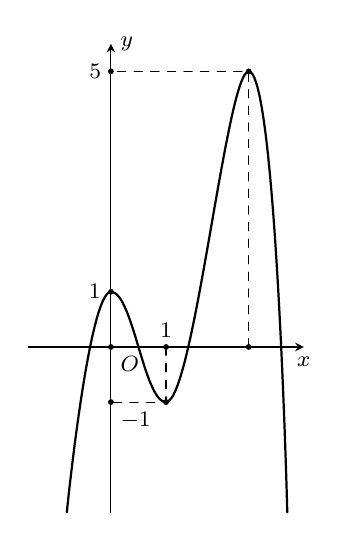
\begin{tikzpicture}[scale=0.7, font=\footnotesize, line join=round, line cap=round, >=stealth]
			\draw[->] (-1.5,0)--(3.5,0)node[below]{$x$};
			\draw[->] (0,-3)--(0,5.5)node[right]{$y$};
			\draw [thick] (-0.8,-3)..controls +(0:0) and +(180:.4)..(0,1)node[left]{$1$}..controls +(0:0.4) and +(180:0.4)..(1,-1)..controls +(0:0.5) and +(180:0.4)..(2.5,5)..controls +(0:0.5) and +(180:0)..(3.2,-3);
			\draw[dashed] (1,0)node[above]{$1$}--(1,-1)--(0,-1)node[below right]{$-1$} (2.5,0)node[above]{$$}--(2.5,5)--(0,5) node[left]{$5$};
			\node at (0,0) [below right]{$O$};
			\fill[black] (0,0) circle (1.5pt);
			\fill[black] (0,1) circle (1.5pt);
			\fill[black] (0,5) circle (1.5pt);
			\fill[black] (0,-1) circle (1.5pt);
			\fill[black] (1,-1) circle (1.5pt);
			\fill[black] (1,0) circle (1.5pt);
			\fill[black] (2.5,5) circle (1.5pt);
			\fill[black] (2.5,0) circle (1.5pt);
			
		\end{tikzpicture}
	\end{center}
	Có bao nhiêu số nguyên $m\in \left[ -30;30\right] $ để hàm số $g(x)=\left[ f(x+m)\right]^2-mf(x+m) $ có đúng $2$ điểm cực đại?
	\choice
	{$38$}
	{$36$}
	{\True $37$}
	{$35$}
	\loigiai{
		Ta có $\lim\limits_{x\to+\infty}g(x)=+\infty\Rightarrow g(x)$ có đúng $2$ điểm cực đại thì $g(x)$ có bảng biến thiên dạng như hình vẽ
		\begin{center}
			
\begin{tikzpicture}[scale=0.7, font=\footnotesize, line join=round, line cap=round, >=stealth]
				\tkzTabInit[nocadre=false,lgt=1.5,espcl=2.5,deltacl=0.6]
				{$x$ /0.6,$g(x)$ /2}
				{$-\infty$,$x_1$,$x_2$,$x_3$,$x_4$,$x_5$,$+\infty$}
				\tkzTabVar{+/$+\infty$,-/$$,+/$$,-/$$,+/$$,-/$$,+/$+\infty$}
				
			\end{tikzpicture}
		\end{center}
		Vậy $g(x)$ có đúng $5$ điểm cực trị khi\\ $g'(x)=2f(x+m)f'(x+m)-mf'(x+m)=f'(x+m)\left[ 2f(x+m)-m\right]=2f'(x+m)\left[ f(x+m)-\dfrac{m}{2}\right]$ đổi dấu đúng $5$ lần $\Leftrightarrow 2f'(t)\left[ f(t)-\dfrac{m}{2}\right]$ đổi dấu đúng $5$ lần $\Leftrightarrow f(t)-\dfrac{m}{2}$ đổi dấu đúng $2$ lần trên $\mathbb{R}\setminus \{0, a, b\} $, trong đó $x=0, x=a, x=b$ là các điểm cực trị của $f(x)$ và đặt $t=x+m$. Dựa vào đồ thị, ta thấy yêu cầu bài toán tương đương
		$$\hoac{&1\le\dfrac{m}{2}<5\\&\dfrac{m}{2}\le-1}\Leftrightarrow \hoac{&2\le m<10\\&m\le-2}\Rightarrow m \in\{-30,\cdots -2,2,\cdots 9\}.$$\\
		Vậy có $29+8=37$ số nguyên $m$ thỏa yêu cầu bài toán.
	}
\end{ex}



\Closesolutionfile{ans}
\inputansbox{10}{ans/ans-Vted-15-2023}